\chapter{Modulation and dead time}
\label{ch:modulation}

\section{Modulation}

The modulating signal of each leg is written as the normalised phase
reference plus a common offset $m_0$:
%
\begin{equation}
  m_k = \frac{v_{kN,\mathrm{ref}}}{\Vdc} + m_0 ,
  \qquad m_k \in [0,1] , \qquad k = 1,2,3 .
\end{equation}
%
The offset is the same in the three legs, so it cancels in the line
voltages and does not reach the load. Its choice gives the different
modulations:
\begin{itemize}
  \item sinusoidal PWM (SPWM): $m_0 = 0.5$;
  \item space-vector PWM (SV-PWM):
        %
        \begin{equation}
          m_0 = \frac{1 - \max(\cdot) - \min(\cdot)}{2} ,
          \label{eq:zero-seq}
        \end{equation}
        %
        where $\max(\cdot)$ and $\min(\cdot)$ are the largest and smallest
        of the three normalised references;
  \item discontinuous PWM: $m_0 = 1 - \max(\cdot)$ (DPWM-MAX) or
        $m_0 = -\min(\cdot)$ (DPWM-MIN). One leg at a time is clamped to a
        rail and does not switch.
\end{itemize}

The converter uses SV-PWM. \Cref{fig:modulanti} shows the three modulating
signals against the triangular carrier.

\begin{figure}[H]
\centering
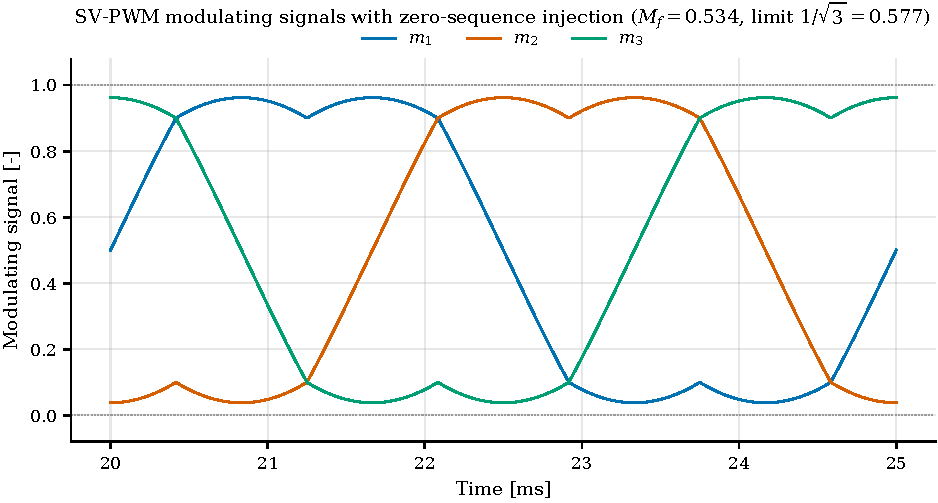
\includegraphics[width=\textwidth]{plecs_05_segnali_modulanti.pdf}
\caption{Modulating signals with the SV-PWM offset of \cref{eq:zero-seq},
against the triangular carrier.}
\label{fig:modulanti}
\end{figure}

\subsection{Choice of the modulation}

\Cref{tab:modulation} and \cref{fig:radar-modulation} compare the three
options.

\begin{table}[H]
\centering
\caption{Carrier-based modulations.}
\label{tab:modulation}
\small
\zebra
\begin{tabularx}{\textwidth}{lYYY}
\toprule
 & SPWM & SV-PWM (chosen) & DPWM \\
\midrule
Offset $m_0$ & 0.5 & $(1-\max-\min)/2$ & $1-\max$ or $-\min$ \\
Maximum linear $M_f$ & 0.500 & 0.577 & 0.577 \\
DC-link utilisation & baseline & +\SI{15.5}{\percent} & +\SI{15.5}{\percent} \\
Switching losses & baseline & baseline & $-\SI{33}{\percent}$ \\
Current ripple & baseline & similar & higher \\
Implementation & simple & one max and one min per period & clamping logic \\
\bottomrule
\end{tabularx}
\end{table}

\begin{figure}[H]
\centering
% Generato da radar.py: non modificare a mano.
\begin{tikzpicture}[font=\footnotesize]
  \draw[black!18] (0.000,0.520) -- (0.495,0.161) -- (0.306,-0.421) -- (-0.306,-0.421) -- (-0.495,0.161) -- cycle;
  \draw[black!18] (0.000,1.040) -- (0.989,0.321) -- (0.611,-0.841) -- (-0.611,-0.841) -- (-0.989,0.321) -- cycle;
  \draw[black!18] (0.000,1.560) -- (1.484,0.482) -- (0.917,-1.262) -- (-0.917,-1.262) -- (-1.484,0.482) -- cycle;
  \draw[black!18] (0.000,2.080) -- (1.978,0.643) -- (1.223,-1.683) -- (-1.223,-1.683) -- (-1.978,0.643) -- cycle;
  \draw[black!40] (0.000,2.600) -- (2.473,0.803) -- (1.528,-2.103) -- (-1.528,-2.103) -- (-2.473,0.803) -- cycle;
  \draw[black!25] (0,0) -- (0.000,2.600);
  \node[align=center, inner sep=2pt, anchor=south] at (0.000,2.782) {DC-link\\utilisation};
  \draw[black!25] (0,0) -- (2.473,0.803);
  \node[align=center, inner sep=2pt, anchor=west] at (2.646,0.860) {low switching\\loss};
  \draw[black!25] (0,0) -- (1.528,-2.103);
  \node[align=center, inner sep=2pt, anchor=west] at (1.635,-2.251) {low current\\ripple};
  \draw[black!25] (0,0) -- (-1.528,-2.103);
  \node[align=center, inner sep=2pt, anchor=east] at (-1.635,-2.251) {low $T_\mathrm{j}$ at\\locked rotor};
  \draw[black!25] (0,0) -- (-2.473,0.803);
  \node[align=center, inner sep=2pt, anchor=east] at (-2.646,0.860) {simple\\implementation};
  \node[black!45, font=\scriptsize, anchor=west] at (0.050,0.520) {1};
  \node[black!45, font=\scriptsize, anchor=west] at (0.050,1.560) {3};
  \node[black!45, font=\scriptsize, anchor=west] at (0.050,2.600) {5};
  \draw[fblu, very thick, fill=fblu, fill opacity=0.12] (0.000,1.560) -- (1.484,0.482) -- (1.223,-1.683) -- (-0.917,-1.262) -- (-2.473,0.803) -- cycle;
  \draw[farancio, very thick, fill=farancio, fill opacity=0.12] (0.000,2.600) -- (1.484,0.482) -- (1.223,-1.683) -- (-0.917,-1.262) -- (-1.978,0.643) -- cycle;
  \draw[fverde, very thick, fill=fverde, fill opacity=0.12] (0.000,2.600) -- (2.473,0.803) -- (0.611,-0.841) -- (-1.528,-2.103) -- (-0.989,0.321) -- cycle;
  \node[anchor=north] at (0,-3.95) {\tikz[baseline=-0.6ex]\draw[fblu, very thick] (0,0) -- (0.45,0); SPWM \quad \tikz[baseline=-0.6ex]\draw[farancio, very thick] (0,0) -- (0.45,0); SV-PWM \quad \tikz[baseline=-0.6ex]\draw[fverde, very thick] (0,0) -- (0.45,0); DPWM};
\end{tikzpicture}

\caption{Modulations compared on a scale from 1 (worst) to 5 (best); a larger area is better.
Utilisation, switching loss and locked-rotor temperature come from the
numbers of this chapter and of \cref{sec:lrdpwm}; the other axes rank the
three options.}
\label{fig:radar-modulation}
\end{figure}

SV-PWM is chosen for these reasons:
\begin{itemize}
  \item It uses \SI{15.5}{\percent} more of the DC-link voltage than SPWM
        ($M_f$ up to 0.577 instead of 0.500), with the same switching loss.
  \item Its current ripple is the same as SPWM.
  \item It needs only the maximum and the minimum of the three references.
\end{itemize}

DPWM would cut the switching loss by about one third. At the rated point
this is about \SI{23}{\watt} of the \SI{70.6}{\watt} of switching
(\cref{tab:losses}) [estimate]. The junction is at \SI{81.8}{\celsius}, so
the rated point does not need this reduction, and DPWM would increase the
current ripple.

At locked rotor DPWM helps more (\cref{sec:lrdpwm}). If the phase at peak
current is clamped, the hottest junction falls from \SI{111.0}{} to
\SI{93.8}{\celsius}. The design, however, does not count on it:
\begin{itemize}
  \item the modulation is set by the controller, which is outside the
        power stage;
  \item every thermal result of this report uses SV-PWM;
  \item DPWM at low output frequency is listed as a recommendation to the
        controller (\cref{tab:sysassume}), and it is an extra margin.
\end{itemize}

\section{Output waveforms}

\begin{figure}[H]
\centering
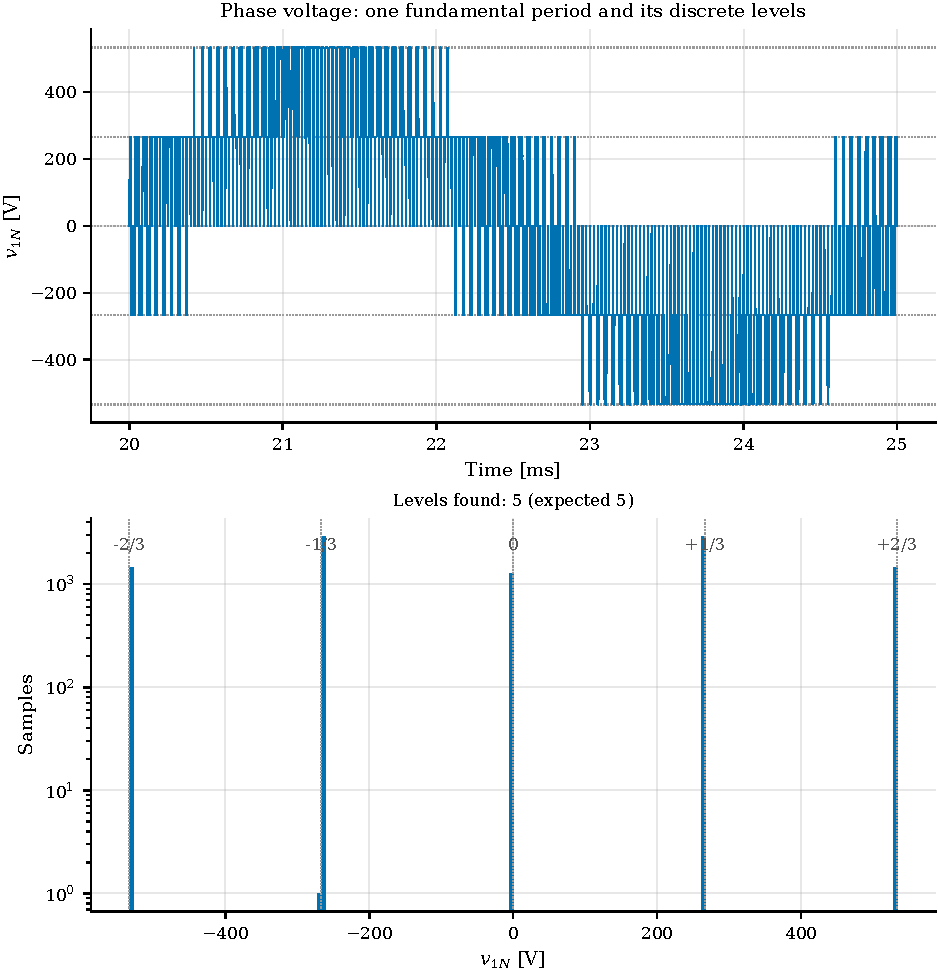
\includegraphics[width=\textwidth]{plecs_02_tensione_di_fase.pdf}
\caption[Phase voltage referred to the load neutral]{Phase voltage $v_{1N}$ referred to the load neutral, with the five
levels $0, \pm\Vdc/3, \pm 2\Vdc/3$.}
\label{fig:tensioni}
\end{figure}

Each pole voltage $v_{k0}$ has only two values, $0$ and $\Vdc$. The load
neutral floats, so the phase voltage $v_{1N} = v_{10} - v_{N0}$ has the five
levels of \cref{fig:tensioni}.

\begin{figure}[H]
\centering
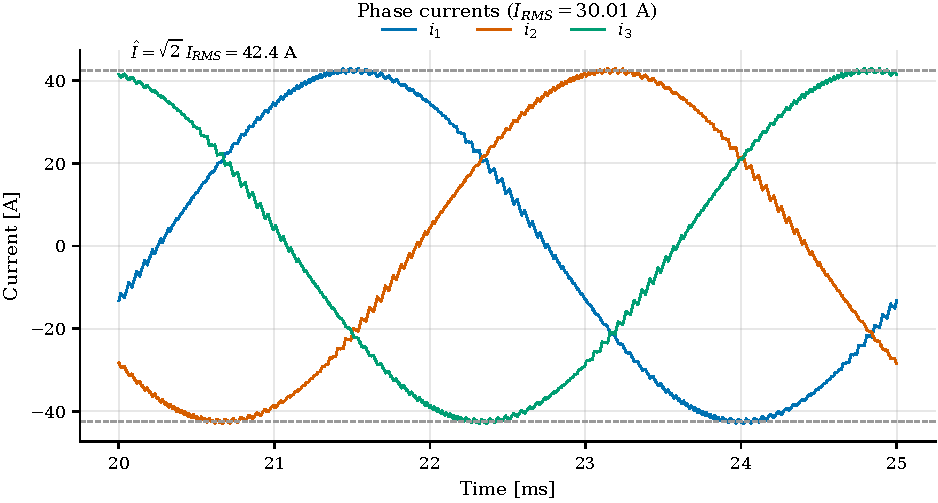
\includegraphics[width=\textwidth]{plecs_03_correnti_di_fase.pdf}
\caption{Phase currents. The switching ripple is \SI{2.463}{\ampere}
peak-to-peak, \SI{5.80}{\percent} of the peak and \SI{0.844}{\percent} in
RMS terms.}
\label{fig:correnti}
\end{figure}

The brief asks for a negligible output current ripple. With the
\SI{2.5}{\milli\henry} load the ripple is:
\begin{itemize}
  \item \SI{2.46}{\ampere} peak-to-peak, \SI{5.8}{\percent} of the peak;
  \item \SI{0.84}{\percent} of the RMS current, equal to the current THD.
\end{itemize}
No output filter is needed. The ripple is inversely proportional to the load
inductance. A motor with a quarter of this inductance would have four times
the ripple and would need an output inductor.

\section{Dead time}
\label{sec:deadtime}

A dead time between the turn-off of one device of a leg and the turn-on of
the other prevents a shoot-through.

\subsection{Sizing}

The worst case is a slow turn-off of one device together with a fast
turn-on of the other. \Cref{tab:deadtime} adds the three contributions:
\begin{itemize}
  \item the difference between the turn-off and turn-on delays of the
        MOSFET;
  \item the pulse-width distortion of the gate signals;
  \item the skew between the gate signals of the two devices.
\end{itemize}

\begin{table}[H]
\centering
\caption{Dead-time budget. Gate-signal tolerances are maxima of a typical
isolated gate driver~\cite{ti_ucc21750}; blue: chosen value.
Device values are typical, read from the switching-time curves
of~\cite{wolfspeed_e3m0016} at the design gate resistances,
\SI{5}{\ohm} at turn-on and \SI{12.5}{\ohm} at turn-off.}
\label{tab:deadtime}
\zebra
\begin{tabular}{lcl}
\toprule
Contribution & Value & Source \\
\midrule
$t_\mathrm{d(off)} - t_\mathrm{d(on)}$ of the MOSFET, $144 - 38$ & \SI{106}{\nano\second} & \cite{wolfspeed_e3m0016} \\
Pulse-width distortion of the gate signals & \SI{30}{\nano\second} & \cite{ti_ucc21750} \\
Skew between the two gate signals & \SI{30}{\nano\second} & \cite{ti_ucc21750} \\
Minimum & \SI{166}{\nano\second} & \\
Minimum with the fall time $t_f = \SI{32}{\nano\second}$ & \SI{198}{\nano\second} & \\
\scelta Chosen & \SI{260}{\nano\second} & factor 1.57 (1.31 with $t_f$) \\
\bottomrule
\end{tabular}
\end{table}

The largest term is the delay of the MOSFET. It grows with the gate
resistance, so the dead time must be checked again whenever $R_g$ changes.
The gate resistances come from the overshoot limit (\cref{sec:kelvin}).

\begin{figure}[H]
\centering
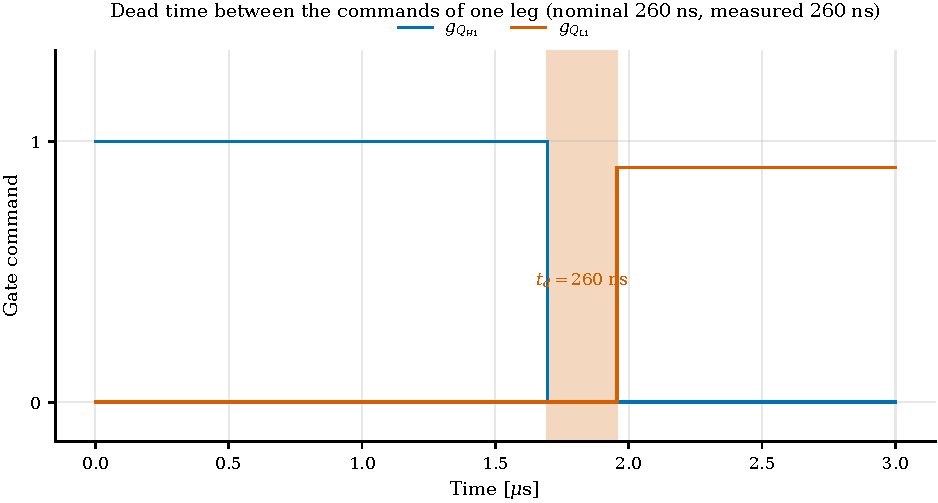
\includegraphics[width=\textwidth]{plecs_06_dead_time.pdf}
\caption{One commutation with the \SI{260}{\nano\second} interval in which
both gate commands are low.}
\label{fig:deadtime}
\end{figure}

\subsection{Loss in the dead time}

During the dead time the phase current flows in the body diode of one
device instead of in its channel. The extra loss is the difference between
the diode drop and the channel drop it replaces:
%
\begin{equation}
  P_\mathrm{dt} = 3 \cdot \big\langle \Delta V(i)\,|i| \big\rangle
  \cdot 2\, t_\mathrm{dead}\, \fsw ,
  \qquad
  \Delta V = V_\mathrm{SD}(i) - v_\mathrm{ch}(i) .
  \label{eq:deadtime-loss}
\end{equation}
%
The factors are:
\begin{itemize}
  \item 3: in each leg one body diode conducts during the dead time,
        chosen by the sign of the phase current;
  \item 2: there are two dead times per switching period;
  \item $\langle\cdot\rangle$: the average over one output period.
\end{itemize}
With the vendor tables of the \device{} at $\Tj = \SI{80}{\celsius}$,
$\Delta V$ averages \SI{3.8}{\volt}. The \SI{260}{\nano\second} dead time
then costs \SI{3.3}{\watt} for the whole converter, about
\SI{2.6}{\percent} of the total loss. \Cref{sec:deadtime-loss} checks this
value with the simulation.
